\subsection*{Modello 4 - small-tune-03 e small-tune-04}


% Introduzione su strategia del training -> qual è l'obiettivo dell'esperimento?


\begin{table}[!htb]
    \centering
    \begin{tabular}{lcc}
        \hline
        \textbf{Iperparametro} & \textbf{Valore st-03} & \textbf{Valore st-04}\\
        \hline
        epoche & 200 & 400 \\
        optimizer & auto (SGD) & Adam \\
        learning rate (lr0) & 0.0001 & 0.0001\\
        learning rate (lrf) & 0.01 & 0.01 \\
        momentum & 0.98 & 0.98\\
        weight\_decay & 0.0005 & 0.0005\\
        imgsz & 800 & 800 \\
        dropout & 0.015 & 0.015 \\
        patience & 100 & 50\\
        \midrule
        hsv\_h & 0.7 & 0.7 \\
        degrees & 120 & 120 \\
        shear & 55 & 55 \\
        \hline
    \end{tabular}
    \caption{Configurazione iperparametri dei modelli \texttt{small-tune-03} e \texttt{small-tune-04} per il training}
    \label{tab:v4-model-configs}
    \end{table}

    
    % Dettagli configurazione, tipologia modello e iperparametri, dove è stato eseguito il train

% Risultati training
% - andamento training

\begin{figure}[!htb]
    \centering
    \includegraphics[width=0.8\textwidth]{v_4/small-tune-03/results.png}
        \caption{Andamento funzioni di loss e metriche durante l'esecuzione di \texttt{small-tune-03}}
        \label{fig:v4-2}
    \end{figure}
    % - grafici recall e precision e performance e F1
    \begin{figure}[!htb]
        \centering
        \begin{subfigure}{.5\textwidth}
            \centering
            \includegraphics[width=.9\linewidth]{v_4/small-tune-03/P_curve.png}
            \subcaption{P-curve}
            \label{fig:v4-3.1}
        \end{subfigure}%
          \begin{subfigure}{.5\textwidth}
            \centering
            \includegraphics[width=.9\linewidth]{v_4/small-tune-03/R_curve.png}
            \subcaption{PR-curve}
            \label{fig:v4-3.2}
        \end{subfigure}
        \vskip\baselineskip
        \begin{subfigure}{.5\textwidth}
            \centering
            \includegraphics[width=.9\linewidth]{v_4/small-tune-03/PR_curve.png}
            \subcaption{PR-curve}
            \label{fig:v4-3.3}
        \end{subfigure}
        \begin{subfigure}{.49\textwidth}
            \centering
            \includegraphics[width=.9\linewidth]{v_4/small-tune-03/F1_curve.png}
            \subcaption{F1-curve}
            \label{fig:v4-3.4}
        \end{subfigure}
        
        \caption{Andamento funzioni di loss e metriche durante l'esecuzione di \texttt{small-tune-03}}
        \label{fig:v4-3}
    \end{figure}
    
  
%----------------------------------

\begin{figure}[!htb]
    \centering
    \includegraphics[width=0.8\textwidth]{v_4/small-tune-04/results.png}
        \caption{Andamento funzioni di loss e metriche durante l'esecuzione di \texttt{small-tune-04}}
        \label{fig:v4-6}
    \end{figure}
    % - grafici recall e precision e performance e F1
    \begin{figure}[!htb]
        \centering
        \begin{subfigure}{.5\textwidth}
            \centering
            \includegraphics[width=.9\linewidth]{v_4/small-tune-04/P_curve.png}
            \subcaption{P-curve}
            \label{fig:v4-5.1}
        \end{subfigure}%
          \begin{subfigure}{.5\textwidth}
            \centering
            \includegraphics[width=.9\linewidth]{v_4/small-tune-04/R_curve.png}
            \subcaption{PR-curve}
            \label{fig:v4-5.2}
        \end{subfigure}
        \vskip\baselineskip
        \begin{subfigure}{.5\textwidth}
            \centering
            \includegraphics[width=.9\linewidth]{v_4/small-tune-04/PR_curve.png}
            \subcaption{PR-curve}
            \label{fig:v4-5.3}
        \end{subfigure}
        \begin{subfigure}{.49\textwidth}
            \centering
            \includegraphics[width=.9\linewidth]{v_4/small-tune-04/F1_curve.png}
            \subcaption{F1-curve}
            \label{fig:v4-5.4}
        \end{subfigure}
        
        \caption{Andamento funzioni di loss e metriche durante l'esecuzione di \texttt{small-tune-04}}
        \label{fig:v4-5}
    \end{figure}

    \begin{table}[!htbp]
        \centering
        \begin{tabularx}{\textwidth}{lYYYc}
            \toprule
            Class & P & R & mAP50 & mAP50-95 \\
            \midrule
            \texttt{small-tune-03} \\
            \midrule
            ALL & 0.450 & 0.451 & 0.382 & 0.170 \\
            PLASTIC\_BAG & 0.436 & 0.428 & 0.394 & 0.157 \\
            PLASTIC\_BOTTLE & 0.672 & 0.769 & 0.731 & 0.333 \\
            OTHER\_PLASTIC\_WASTE & 0.113 & 0.320 & 0.0934 & 0.0353 \\
            NOT\_PLASTIC\_WASTE & 0.576 & 0.288 & 0.311 & 0.154 \\
            \midrule
            \texttt{small-tune-04} \\
            \midrule
            ALL & 0.457 & 0.449 & 0.382 & 0.172 \\
            PLASTIC\_BAG & 0.405 & 0.412 & 0.352 & 0.122 \\
            PLASTIC\_BOTTLE & 0.701 & 0.776 & 0.753 & 0.349 \\
            OTHER\_PLASTIC\_WASTE & 0.131 & 0.345 & 0.102 & 0.0373 \\
            NOT\_PLASTIC\_WASTE & 0.590 & 0.261 & 0.322 & 0.181 \\
            \bottomrule
        \end{tabularx}
        \caption{Risultati delle metriche sul test set per \texttt{small-tune-03} sopra e \texttt{small-tune-03} sotto}
        \label{table:v4-1}
    \end{table}

    % - matrici di confusione
    \begin{figure}[!htb]
        \centering
        \begin{subfigure}{.49\textwidth}
            \includegraphics[width=0.9\textwidth]{v_4/small-tune-03/confusion_matrix_normalized.png}
            \subcaption{\texttt{small-tune-03}}
            \label{fig:v4-4.1}
        \end{subfigure}
        \begin{subfigure}{.49\textwidth}
            \includegraphics[width=0.9\textwidth]{v_4/small-tune-04/confusion_matrix_normalized.png}
            \subcaption{\texttt{small-tune-04}}
            \label{fig:v4-4.1}
        \end{subfigure}
        \caption{Matrice di confusione normalizzata data dai due modelli \texttt{small-tune-03} e \texttt{small-tune-04}}
        \label{fig:v4-4}
    \end{figure}
    % - tabella performance test set

